%!TEX root=../main.tex
\section{Empirical analysis} % (fold)
\label{sec:empirical_analysis}

Using simulated data, in this Section, we compare the behavior of the estimation of the eigencomponents using the diagonalisation of the covariance operator and the Gram matrix. The diagonalisation of the covariance operator is performed using the methodology of \cite{happMultivariateFunctionalPrincipal2015}. As this methodology is based on the expansion of each univariate components, we used univariate FPCA if the curves are unidimensional and the FCP-TPA algorithm for regularized tensor decomposition \citep{allenMultiwayFunctionalPrincipal2013a}, if the curves are two-dimensional. We choose to use the FCP-TPA algortihm as it is the one used by \cite{happMultivariateFunctionalPrincipal2015} in their algorithm and implemented in their software \citep{happ-kurzObjectOrientedSoftwareFunctional2020}. Note that we could also use a two-dimensional basis expansion such as penalized tensor splines or discrete cosine transform, but we do not investigate this expansion here, as we do not want to prespecify a basis of functions.

We are greatly interested in the ability of the methods to retrieve the right number of components $K$ for a given percentage of variance explained.

\textcolor{red}{**************}

We run simulations to check the goodness of fit of the MFPCA using both methods and compare the time complexity of the two ways. 

Some ideas:
\begin{itemize}
    \item Varies number of curves in the sample $N = 50, 100, 200$.
    \item Varies number of points per curve $M = 20, 50, 100$.
    \item Varies number of components $P = 1, 5, 10, \dots$.
    \item Common grid / Irregularly sampled grid. If the grid is common but not equally spaced, e.g., the axis is log-transformed, we have to be careful on the integration part / integration weights. This is an important part of FDA, as if the curve are densely sampled on a common grid, there is not much difference as with usual statistical methodologies. In the FDA settings, we can have that sort of settings. 
    \item Denoising
\end{itemize}

\textcolor{red}{Not true anymore. For all settings, we consider that the curves are centered such that $\mu = 0$. We generate covariance matrices $\Gamma$ using Mercer's theorem. We generate samples of independent paths $X_i$ from the Gaussian process characterized by $\mu$ and $\Gamma$.}

We consider \textcolor{red}{some number} of experiments, each of them replicated $500$ times.

The results of the simulation are compared using computation times, the integrated squared error (ISE) risk for the multivariate eigenfunctions and the mean squared error (MSE) risk for the eigenvalues and the mean integreated squared error (MISE) risk for the reconstructed data.

\textcolor{red}{Definition ISE for eigenfunctions}
Let $\psi$ be the true eigenfunction and $\widehat{\psi}$ the estimated eigenfunction defined on $\TT{}$. We then defined the ISE as 
\begin{equation}\label{eq:ise_eigenfunctions}
    \text{ISE}(\psi, \widehat{\psi}) = \normH{\psi - \widehat{\psi}}^2 = \sum_{p = 1}^P \int_{\TT{p}} \{\psi^{(p)}(t) - \widehat{\psi}^{(p)}(t)\}^2 \dd t.
\end{equation}
Might also want to define a version of the ISE without the boundaries.

\textcolor{red}{Definition MSE for eigenvalues}
Let $\lambda = (\lambda_1, \dots, \lambda_K)$ be the vector of true eigenvalues and $\widehat{\lambda} = (\widehat{\lambda}_1, \dots, \widehat{\lambda}_K)$ be the vector of estimated eigenvalues. We then define the MSE as 
\begin{equation}\label{eq:mse_eigenvalues}
    \text{MSE}(\lambda, \widehat{\lambda}) = \sum_{k = 1}^K \frac{\widehat{\lambda}_k}{\lambda_k}.
\end{equation}

\textcolor{red}{Definition MISE for reconstructed data}
Let $\mathcal{X}$ be the set of true data and $\widehat{\mathcal{X}}$ be the set of reconstructed data. We defined the MISE as
\begin{equation}\label{eq:mise_reconstructed_data}
    \text{MISE}(\mathcal{X}, \widehat{\mathcal{X}}) = \frac{1}{N}\sum_{n = 1}^N \normH{X_n - \widehat{X}_n}^2 = \frac{1}{N}\sum_{n = 1}^N \sum_{p = 1}^P \int_{\TT{p}} \left\{\Xnp - \hatXnp \right\}^2 \dd t.
\end{equation}

Consider the simulations in \cite{happMultivariateFunctionalPrincipal2015} as example.

We first consider curves observed without noise and a common and regularly spaced grid. For 2D data, we compare the decomposition of the Gram matrix with the FCP-TPA algorithm \cite{allenMultiwayFunctionalPrincipal2013a}. We choose to compare with this algorithm because it is the one that is proposed in \cite{happMultivariateFunctionalPrincipal2015} to compute the MFPCA where some components are 2D and the one that is implemented in their software \citep{happ-kurzObjectOrientedSoftwareFunctional2020}. Note that we could also use a 2D basis expansion such as penalized tensor splines or discrete cosine transform, but we do not investigate this expansion here, as we do not want to prespecify a basis of functions.

\subsection{Simulation settings} % (fold)
\label{sub:simulation_settings}

The simulation settings are based on the simulation in \cite{happMultivariateFunctionalPrincipal2015}. For data on one-dimensional domains, the data generating process is based on a truncated version of the Karhunen-Loève decomposition. First, we generate a large orthonormal basis $\{\phi_k\}_{k \in \NN}$ of $\sLp{\TT{}}$ on an interval $\TT{} = [0, T] \subset \RR$. We define $P$ cutting points $T_1, \dots, T_P$ in $\TT{}$, $\eta_1, \dots, \eta_P \in \RR$ and $\sigma_1, \dots, \sigma_P \in \{-1, 1\}$. The univariate components are defined as
\begin{equation}\label{eq:simulation_uni_component}
    \psi_k^{(p)}(t_p) = \sigma_p \restr{\phi_k}{[T_p, T_{p + 1}]}(t_p - \eta_p), \quad k = 1, \dots, K.
\end{equation}
The set of functions $\{\psi_k, k = 1, \dots, K\}$ is an orthonormal system in $\HH \coloneqq \sLp{\TT{1}} \times \dots \times \sLp{\TT{P}}$ with $\TT{p} = [T_p + \eta_p, T_{p + 1} + \eta_p]$.

For images data, the eigenfunctions are simulated using the truncated Karhunen-Loève decomposition. The images basis of functions is build on a tensor product of an orthonormal basis of functions. \textcolor{red}{From Ed: Just a quick note here. I think that this construction implies so-called "weak separability" of the process X(s, t) (Chen and Lynch, 2017). I wonder if Happ's FPCA-TPA can even work if this assumption doesn't hold, i.e., if we generate data from a non-separable process. Once way to do it would be to expand each coefficient of one dimensions basis in a unique basis of the other dimension!}

The scores are generated as independent realisations of a Gaussian distribution with mean $0$ and variance $\lambda_k$. We use an exponential decreasing of the eigenvalues.

\subsection{Simulation results} % (fold)
\label{sub:simulation_results}

\begin{figure}
    \centering
    \includegraphics[scale=0.25]{figures/mise_pall.eps}
    \caption{MISE for multivariate functional data. Each univariate component is defined on a one-dimensional domain. \textcolor{red}{to be modify}}
    \label{fig:mise_mfd_1d}
\end{figure}

\begin{figure}
    \centering
    \includegraphics[scale=0.25]{figures/mise_p1.eps}
    \caption{MISE for 2D data \textcolor{red}{to be modify}}
    \label{fig:mise_fd_2d}
\end{figure}

% subsection simulation_results (end)


\subsection{Computation time} % (fold)
\label{sub:computation_time}

\begin{figure}
    \centering
    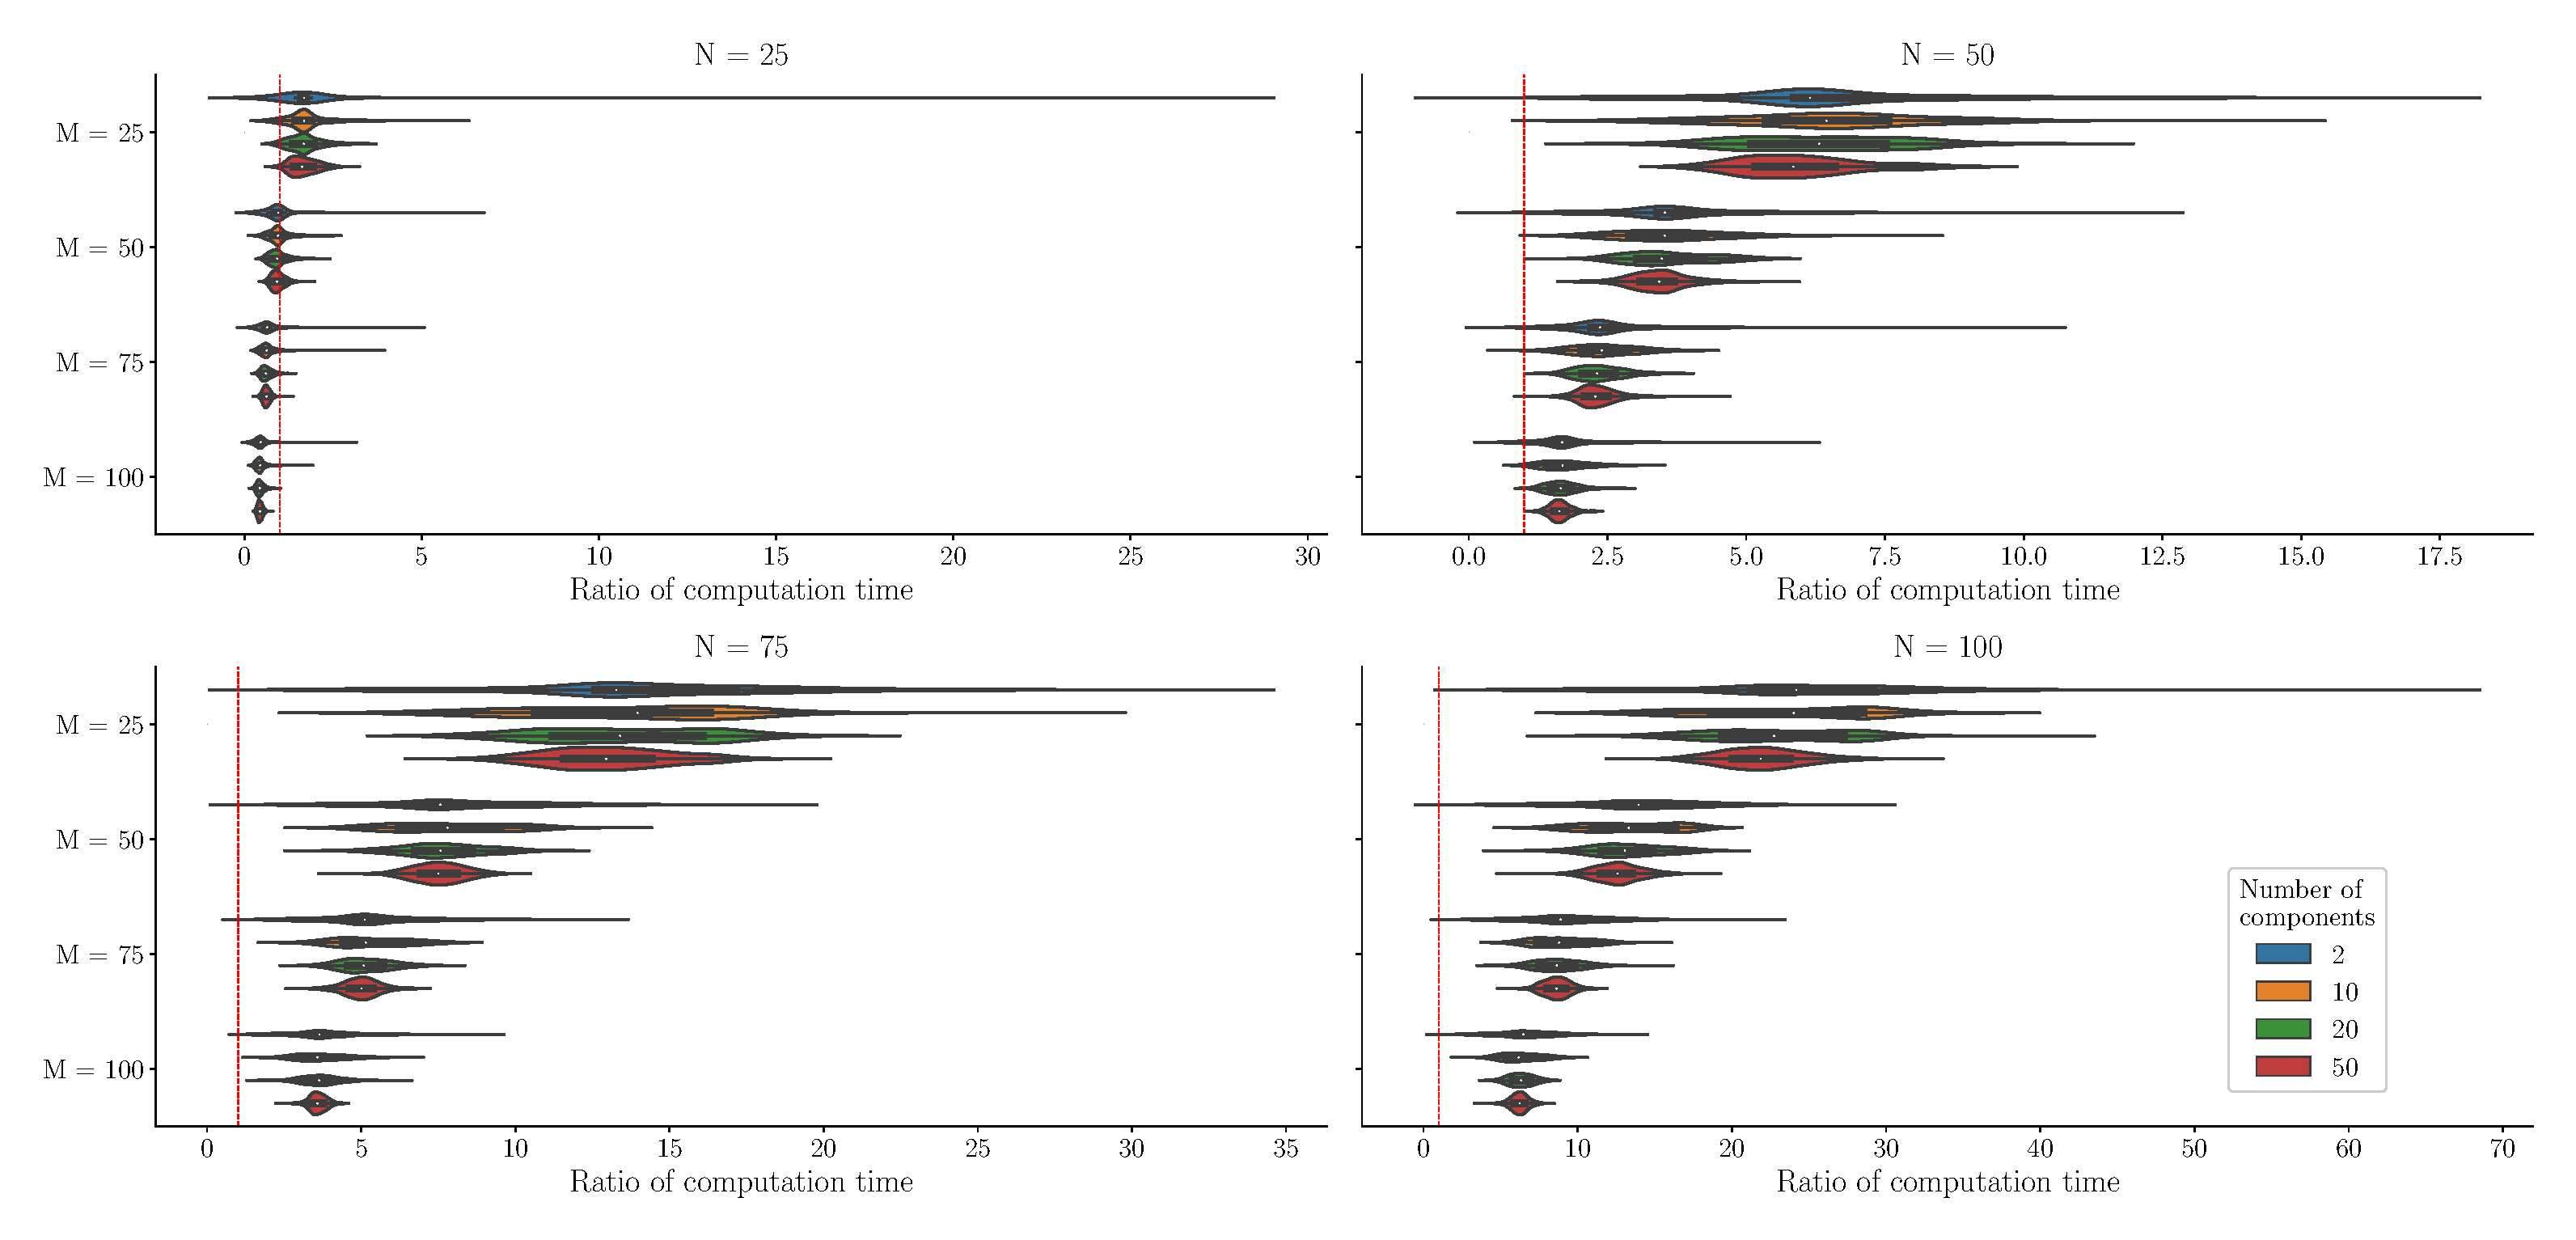
\includegraphics[scale=0.25]{figures/computation_time_pall.eps}
    \caption{Computation time for multivariate functional data. Each univariate component is defined on a one-dimensional domain. \textcolor{red}{to be modify}}
    \label{fig:computation_time_mfd_1d}
\end{figure}

\begin{figure}
    \centering
    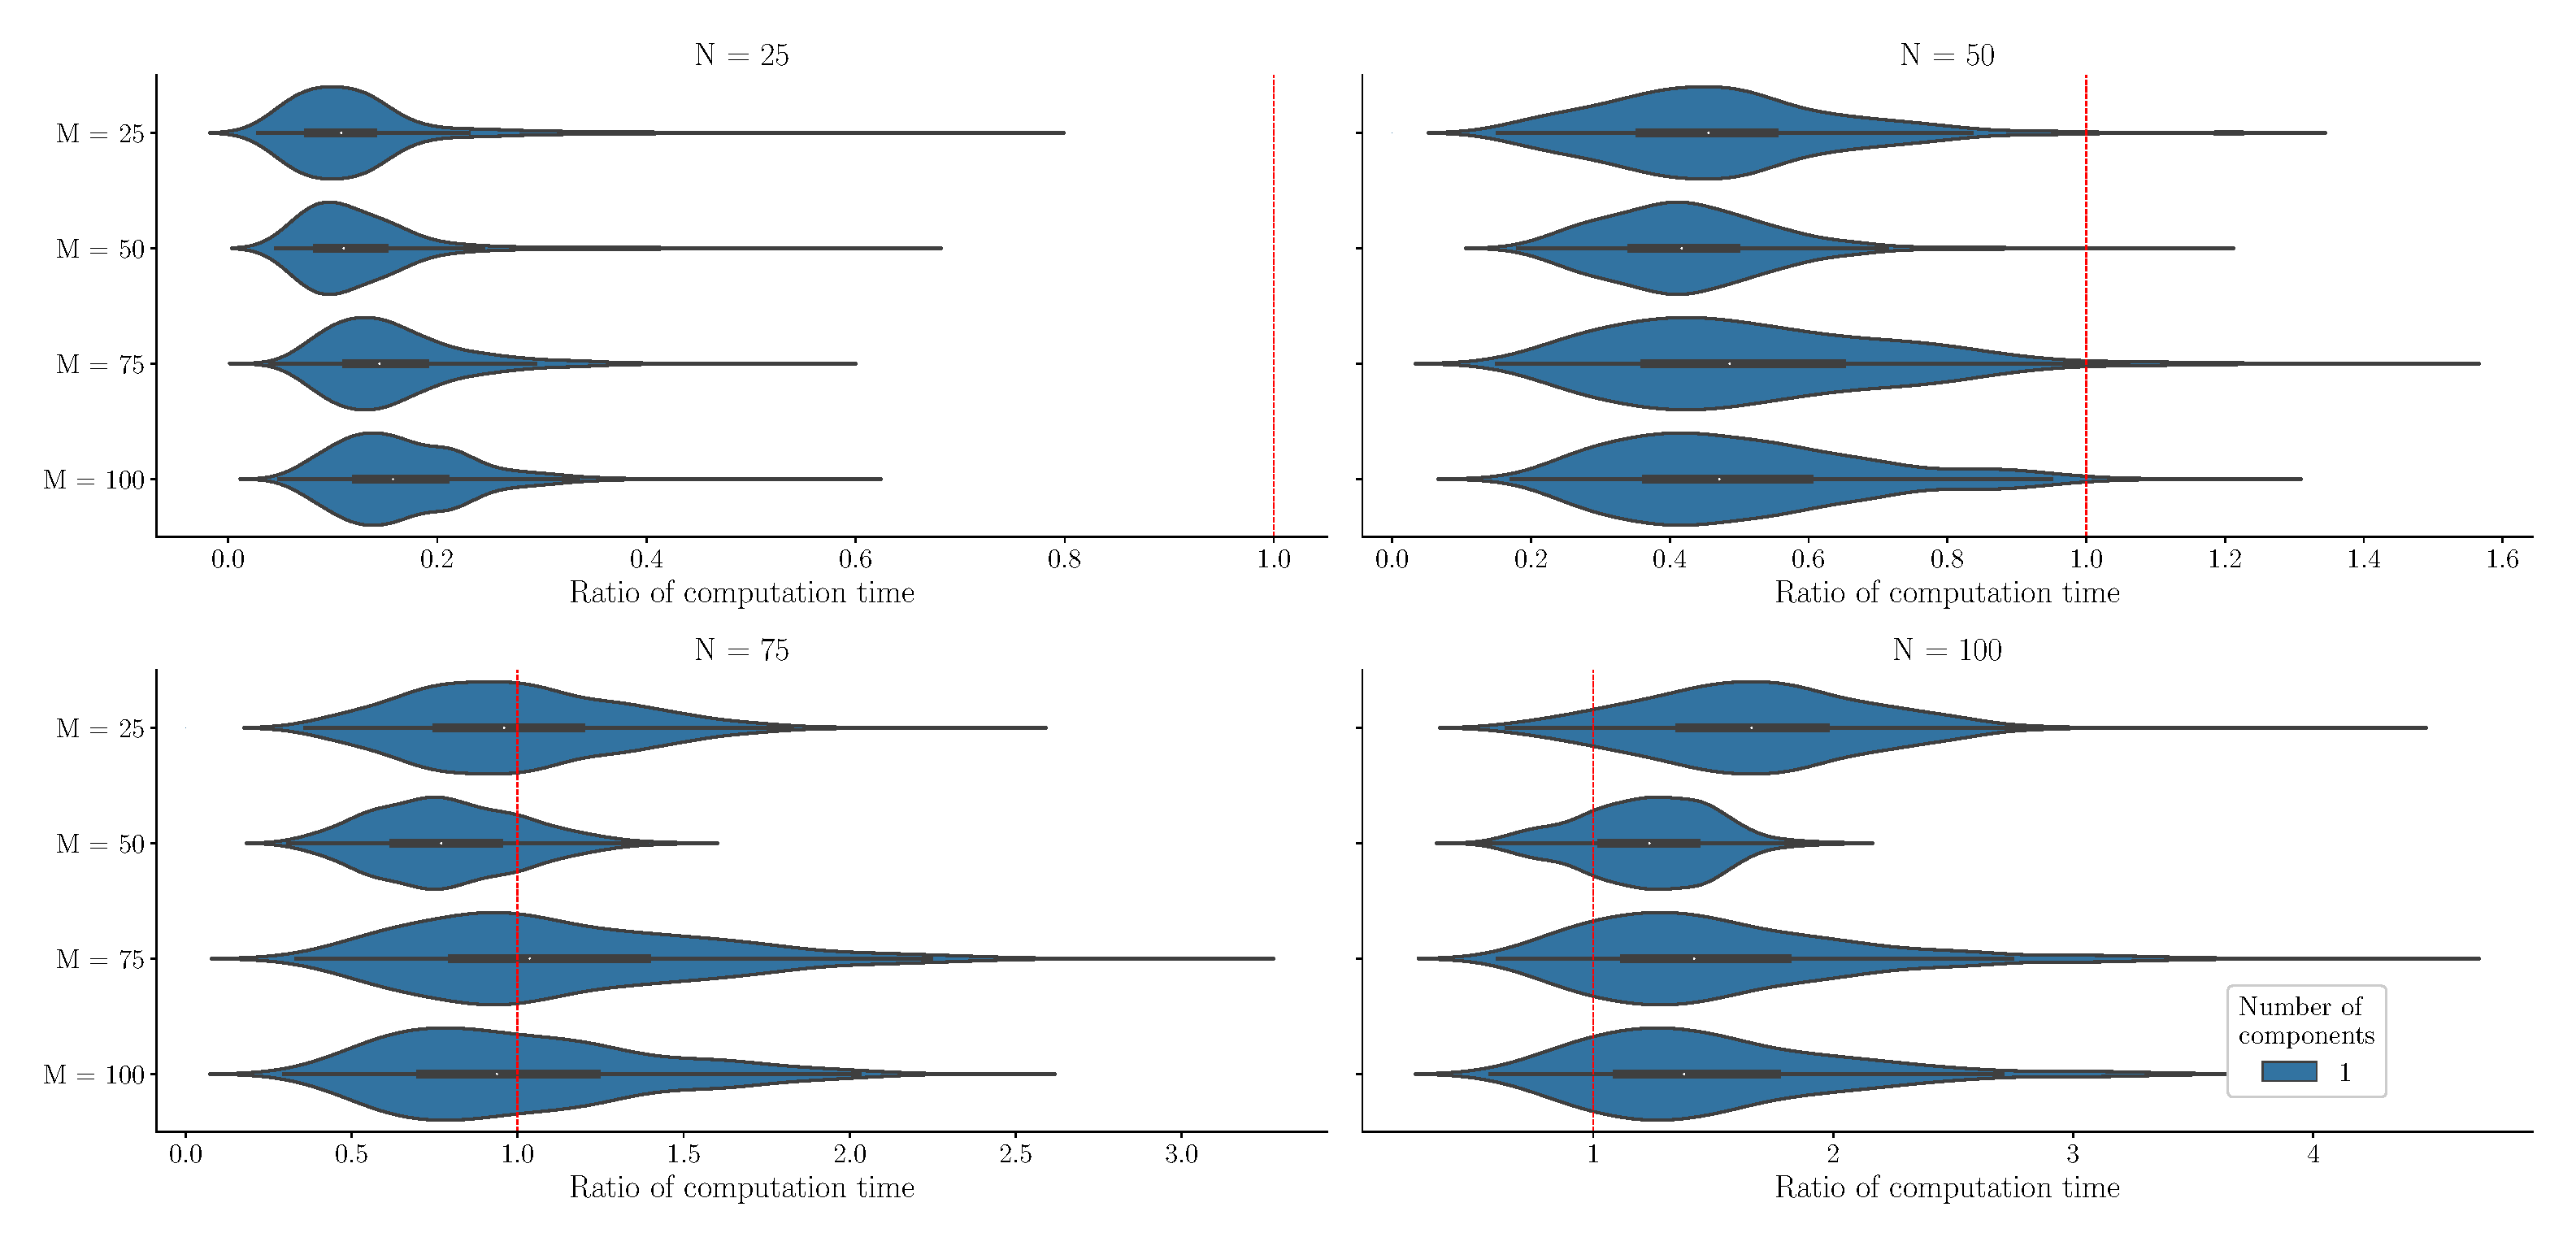
\includegraphics[scale=0.25]{figures/computation_time_p1.eps}
    \caption{Computation time for univariate functional data of images data \textcolor{red}{to be modify}}
    \label{fig:computation_time_fd_2d}
\end{figure}

% subsection computation_time (end)


% subsection simulation_settings (end)

\subsection{Percentage of variance explained} % (fold)
\label{sub:percentage_of_variance_explained_simulation}

We show that choosing a univariate cut-off within each univariate dimension (e.g, $95\%$) does not lead to the same percentage of variance explained for the multivariate functions.

We consider the following settings of simulation. Using the multivariate Karhunen-Loève theorem, we generate

\begin{equation}\label{eq:simu_var_explained}
\begin{pmatrix} \Xp{1} \\ \Xp{2} \end{pmatrix} = \sum_{k = 1}^{20} \mathfrak{c}_k \begin{pmatrix} \psi_k^{(1)} \\ \psi_k^{(2)} \end{pmatrix},
\end{equation}
where $\{\psi_k^{(1)}\}_{k = 1, \dots, 20}$ are the first $20$ functions of the Fourier basis and $\{\psi_k^{(2)}\}_{k = 1, \dots, 20}$ are the first $20$ functions of the Wiener basis, the coefficients $\mathfrak{c}_k$ are generated independently from a Gaussian distribution with mean $0$ and variance $\lambda_k$. We consider linear and exponential decreasing of the eigenvalues.

The true percentage of variance explained by the $k$th component is given by
$\lambda_k / \sum_{k^\prime = 1}^{20} \lambda_{k\prime}$. The true percentage of variance explained by the first $K$ components is given by $\sum_{k = 1}^K \lambda_k / \sum_{k^\prime = 1}^{20} \lambda_{k\prime}$.

We fix a certain percentage of variance explained $\alpha$. To compare the estimation of the estimation of the number of components needed to reach $\alpha$, we first run FPCA on each univariate components to estimate the number of components needed to explain $\alpha\%$ of the variance for each components. Then, we run an MFPCA with the number of components equal to the sum of the univariate components. We finally compare the estimated number of components with the true one and the total variance explained.

Using the Gram matrix, we directly estimated the number of components needed to explain $\alpha\%$ of the variance of the multivariate functional data.

% subsection percentage_of_variance_explained (end)

\subsection{Noisy data} % (fold)
\label{sub:noisy_data}

We consider noisy dataset. We simulate datasets are the same as before except we add a random noise as an independent Gaussian variable with mean $0$ and variance $\sigma^2$ to the curve.

\begin{equation}\label{eq:noisy_curves}
    Y(t) = X(t) + \varepsilon(t)
\end{equation}

% subsection noisy_data (end)

% section empirical_analysis (end)